\subsection{Area 4 – Consultazione e cancellazione delle prenotazioni}
\begin{figure}[H]
\centering
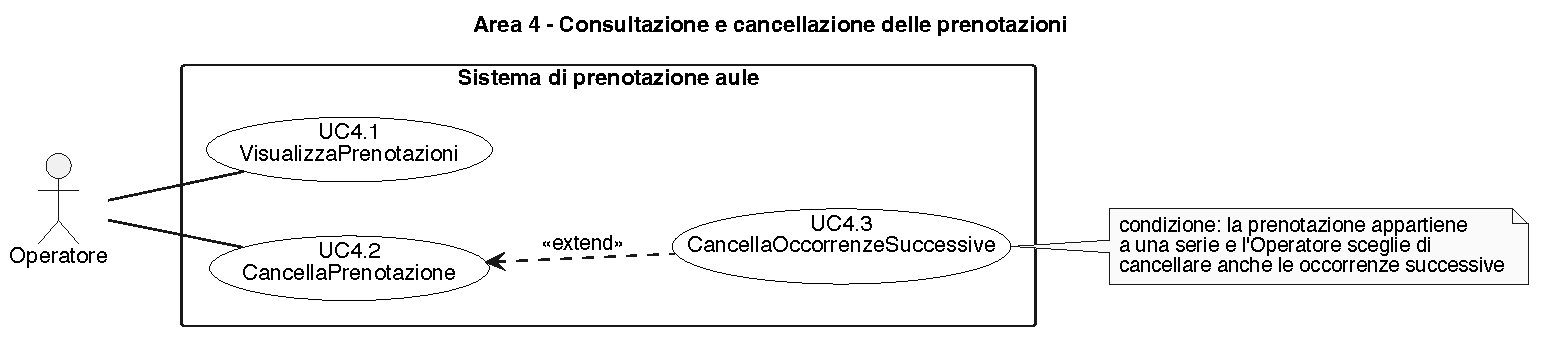
\includegraphics[width=\textwidth,height=0.8\textheight,keepaspectratio]{diagrammi/uc-area4-consultazione}
\caption{Casi d'uso dell'Area 4 – Consultazione e cancellazione delle prenotazioni}
\end{figure}

\subsubsection{[UC4.1] VisualizzaPrenotazioni}
\noindent Attore: Operatore\\
Requisiti correlati: FI4.1, FI4.2, FI4.3, IU4.1, IU4.2, IU4.8\\
Pre-condizioni: Nessuna oltre alla precondizione comune.\\
Post-condizioni: Il sistema mostra le prenotazioni che soddisfano gli eventuali filtri, ordinate per data e ora di inizio. L'archivio è invariato.\\

\noindent Flusso principale:
\begin{enumerate}
\item L'Operatore apre la sezione Prenotazioni.
\item Il sistema mostra tutte le prenotazioni ordinate per data e ora di inizio (a parità, per codice dell'aula), con data, orari, aula, docente, tipo, denominazione e indicazione ``ricorrente''.
\item L'Operatore sceglie un'aula e/o un docente come filtro.
\item Il sistema mostra solo le prenotazioni che soddisfano tutti i filtri impostati, mantenendo l'ordine.
\end{enumerate}
\noindent Flussi alternativi:
\begin{itemize}
\item \textbf{2a.} Non è registrata nessuna prenotazione:
\begin{itemize}
\item 2a.1 Il sistema mostra la tabella vuota con il messaggio ``Nessuna prenotazione registrata'' e il caso d'uso termina.
\end{itemize}
\item \textbf{4a.} Nessuna prenotazione soddisfa i filtri:
\begin{itemize}
\item 4a.1 Il sistema mostra la tabella vuota con il messaggio ``Nessuna prenotazione corrisponde ai filtri''.
\end{itemize}
\item \textbf{4b.} L'Operatore rimuove i filtri:
\begin{itemize}
\item 4b.1 si riprende dal passo 2.
\end{itemize}
\end{itemize}

\subsubsection{[UC4.2] CancellaPrenotazione}
\noindent Attore: Operatore\\
Requisiti correlati: FI4.4, IU4.3, IU4.5, IU4.7\\
Pre-condizioni: Il sistema mostra la sezione Prenotazioni e nell'archivio è registrata almeno una prenotazione.\\
Post-condizioni: La prenotazione selezionata è rimossa dall'archivio e l'archivio è salvato su file. Se era un'occorrenza di una serie, le altre occorrenze restano invariate.\\
Punto di estensione: Passo 3: la prenotazione appartiene a una serie e l'Operatore sceglie ``Questa e tutte le successive'' $\rightarrow$ UC4.3 CancellaOccorrenzeSuccessive.\\

\noindent Flusso principale:
\begin{enumerate}
\item L'Operatore seleziona una prenotazione nella lista e sceglie il comando Cancella.
\item Il sistema verifica che la prenotazione non sia conclusa.
\item La prenotazione non appartiene a una serie: il sistema chiede conferma mostrando i dati della prenotazione (IU4.3).
\item L'Operatore conferma.
\item Il sistema rimuove la prenotazione, salva l'archivio e mostra la lista aggiornata con un messaggio di esito.
\end{enumerate}
\noindent Flussi alternativi:
\begin{itemize}
\item \textbf{1a.} L'Operatore sceglie Cancella senza aver selezionato una prenotazione:
\begin{itemize}
\item 1a.1 Il sistema chiede di selezionare una prenotazione;
\item 1a.2 si riprende dal passo 1.
\end{itemize}
\item \textbf{2a.} La prenotazione è conclusa:
\begin{itemize}
\item 2a.1 Il sistema segnala che le prenotazioni concluse non possono essere cancellate e il caso d'uso termina.
\end{itemize}
\item \textbf{3a.} La prenotazione è un'occorrenza di una serie:
\begin{itemize}
\item 3a.1 Il sistema chiede se cancellare ``Solo questa occorrenza'' o ``Questa e tutte le successive'' (IU4.5);
\item 3a.2 se l'Operatore sceglie ``Solo questa occorrenza'', si prosegue dal passo 4;
\item 3a.3 se l'Operatore sceglie ``Questa e tutte le successive'', si esegue UC4.3 CancellaOccorrenzeSuccessive e il caso d'uso termina.
\end{itemize}
\item \textbf{4a.} L'Operatore annulla: si applica FC1.
\item \textbf{5a.} Il salvataggio non riesce: si applica FC2.
\end{itemize}

\subsubsection{[UC4.3] CancellaOccorrenzeSuccessive}
\noindent Attore: Operatore\\
Requisiti correlati: FI4.5, IU4.5, IU4.7, ED3.7\\
Estende: UC4.2 CancellaPrenotazione, quando la prenotazione selezionata appartiene a una serie e l'Operatore sceglie di cancellare anche le occorrenze successive.\\
Pre-condizioni: L'Operatore ha selezionato un'occorrenza non conclusa di una serie e ha scelto ``Questa e tutte le successive''.\\
Post-condizioni: L'occorrenza selezionata e tutte le occorrenze successive della stessa serie sono rimosse dall'archivio e l'archivio è salvato su file. Le occorrenze precedenti restano invariate.\\

\noindent Flusso principale:
\begin{enumerate}
\item Il sistema mostra l'elenco delle occorrenze che verranno rimosse (l'occorrenza selezionata e le successive della stessa serie), con data, orari e numero totale, e chiede conferma.
\item L'Operatore conferma.
\item Il sistema rimuove le occorrenze elencate, salva l'archivio e mostra la lista aggiornata con un messaggio con il numero di occorrenze rimosse.
\end{enumerate}
\noindent Flussi alternativi:
\begin{itemize}
\item \textbf{2a.} L'Operatore annulla: si applica FC1.
\item \textbf{3a.} Il salvataggio non riesce: si applica FC2.
\end{itemize}
